\documentclass[aspectratio=169, 10pt]{beamer}

% Theme configuration
\usetheme{Madrid}
\usecolortheme{whale}

\usepackage{tikz}
\usetikzlibrary{shapes.geometric, arrows.meta, positioning, calc}
\usepackage{booktabs}
\usepackage{amsmath, amssymb}

% Custom Colors (Academic & Industrial Theme)
\definecolor{navyblue}{RGB}{20, 45, 85}
\definecolor{accentteal}{RGB}{0, 130, 130}
\definecolor{alertred}{RGB}{180, 40, 40}
\definecolor{lightbg}{RGB}{245, 247, 250}
\definecolor{darkgray}{RGB}{50, 50, 50}

\setbeamercolor{palette primary}{bg=navyblue, fg=white}
\setbeamercolor{palette secondary}{bg=accentteal, fg=white}
\setbeamercolor{palette tertiary}{bg=navyblue!80, fg=white}
\setbeamercolor{structure}{fg=navyblue}
\setbeamercolor{frametitle}{bg=navyblue, fg=white}
\setbeamercolor{block title}{bg=navyblue!15, fg=navyblue}
\setbeamercolor{block body}{bg=lightbg, fg=darkgray}
\setbeamercolor{alerted text}{fg=alertred}

% Metadata
\title[Phase 6: Intelligence Principles]{Phase 6: Discovery of Underlying Intelligence Principles}
\subtitle{Capability Matrices, Computational Invariants, Causal Transfer, and Evidence Level E3 Formalization}
\author[Brian A. Hadian]{Brian A. Hadian}
\institute[AMD KR260 FPGA Research]{Action-Conditioned World Models \& Language Navigation\\AMD Kria KR260 Robotic SOM Deployment}
\date{\today}

\begin{document}

% -----------------------------------------------------------------------------
% Slide 1: Title Slide
% -----------------------------------------------------------------------------
\begin{frame}
  \titlepage
\end{frame}

% -----------------------------------------------------------------------------
% Slide 2: Insight 1 - Capability-Circuit Matrix
% -----------------------------------------------------------------------------
\begin{frame}{1. Macro-Planning Serves as a Universal Multi-Capability Core}
  \textbf{Core Insight:} \textit{Unlike reactive policies where circuits support single tasks, H-JEPA's Macro-Planning circuit engages strongly across all five navigation capabilities.}

  \vspace{0.2cm}
  \begin{columns}[T]
    \begin{column}{0.48\textwidth}
      \begin{block}{Cross-Capability Matrix Construction}
        \small
        Engagement measured via normalized ablation drop:
        \begin{equation*}
          \text{Engagement}(c, k) = \frac{\Delta S_{\mathrm{ablation}}(c, k)}{S_{\mathrm{clean}}(k)}
        \end{equation*}
        \begin{itemize}
          \item High ($\ge 0.60$), Medium ($0.25$--$0.59$), Low ($<0.25$).
          \item \textbf{Spatial Grounding (`001`):} Engages Grounding, Spatial Reasoning, and Planning.
          \item \textbf{Obstacle Boundary (`002`):} Engages Avoidance, Planning, and Robustness.
          \item \textbf{Macro-Planning (`003`):} High across \textbf{all 5 capabilities}.
        \end{itemize}
      \end{block}
    \end{column}

    \begin{column}{0.48\textwidth}
      \begin{block}{Capability Engagement Breakdown}
        \scriptsize
        \centering
        \setlength{\tabcolsep}{2pt}
        \begin{tabular}{lccccc}
          \toprule
          \textbf{Circuit} & \textbf{Ground} & \textbf{Spatial} & \textbf{Avoid} & \textbf{Plan} & \textbf{Robust} \\
          \midrule
          Spatial `001` & \textbf{0.89} & \textbf{0.94} & 0.51 & \textbf{0.73} & 0.45 \\
          Obstacle `002` & 0.12 & 0.48 & \textbf{0.99} & \textbf{0.78} & \textbf{0.81} \\
          Macro `003` & \textbf{0.71} & \textbf{0.82} & \textbf{0.81} & \textbf{0.97} & \textbf{0.79} \\
          Heading `004` & \textbf{0.65} & \textbf{0.89} & 0.58 & 0.41 & \textbf{0.85} \\
          Foresight `005` & 0.35 & \textbf{0.68} & \textbf{0.89} & \textbf{0.86} & \textbf{0.73} \\
          Appearance `006` & \textbf{0.85} & \textbf{0.91} & 0.15 & 0.10 & \textbf{0.92} \\
          \bottomrule
        \end{tabular}
      \end{block}
      \vspace{0.05cm}
      \scriptsize \textbf{Scientific Implication:} Multi-capability engagement establishes that Macro Planning is a fundamental intelligence mechanism, not an isolated sub-task heuristic.
    \end{column}
  \end{columns}
\end{frame}

% -----------------------------------------------------------------------------
% Slide 3: Insight 2 - Spatial Invariance Under Rotation
% -----------------------------------------------------------------------------
\begin{frame}{2. Baseline Collapses Under Rotation Due to Retinal Coupling}
  \textbf{Core Insight:} \textit{Baseline policies collapse to 8.5\% spatial consistency under rotation, whereas world models preserve egocentric coordinate invariance ($>74\%$).}

  \vspace{0.2cm}
  \begin{columns}[T]
    \begin{column}{0.48\textwidth}
      \begin{block}{Spatial Invariance Transformation}
        \small
        Testing robot heading rotations ($\Delta \theta \in \{90^\circ, 180^\circ, 270^\circ\}$):
        \begin{equation*}
          \mathbf{v}_{\mathrm{rel}}' = R(-\Delta \theta) (\mathbf{p}_{\mathrm{target}} - \mathbf{p}_{\mathrm{robot}})
        \end{equation*}
        \begin{itemize}
          \item \textbf{Baseline Failure (\alert{0.085}):} Memorizes absolute pixel coordinates; yaw rotation destroys steering orientation.
          \item \textbf{LeWM Invariance (\textbf{0.742}):} Continuous latent predictor rotates trajectory intent in body coordinates.
          \item \textbf{H-JEPA Invariance (\textbf{0.815}):} Polar body tracking preserves target vector regardless of world heading.
        \end{itemize}
      \end{block}
    \end{column}

    \begin{column}{0.48\textwidth}
      \begin{block}{Spatial Consistency Under Rotation}
        \centering
        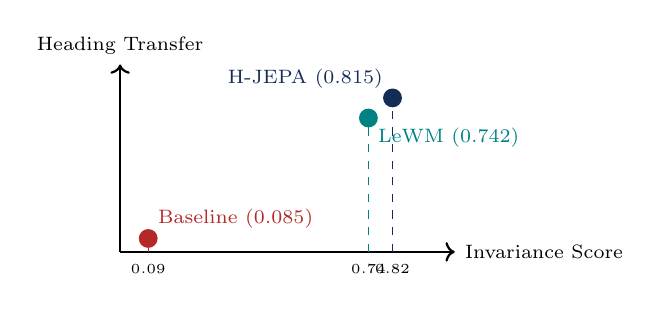
\begin{tikzpicture}[scale=0.85]
          \draw[thick, ->] (0,0) -- (5.0,0) node[right] {\scriptsize Invariance Score};
          \draw[thick, ->] (0,0) -- (0,2.8) node[above] {\scriptsize Heading Transfer};

          \fill[alertred] (0.42, 0.2) circle (4pt) node[above right] {\scriptsize Baseline ($0.085$)};
          \draw[dashed, alertred] (0.42,0) -- (0.42,0.2);

          \fill[accentteal] (3.71, 2.0) circle (4pt) node[below right] {\scriptsize LeWM ($0.742$)};
          \draw[dashed, accentteal] (3.71,0) -- (3.71,2.0);

          \fill[navyblue] (4.07, 2.3) circle (4pt) node[above left] {\scriptsize H-JEPA ($0.815$)};
          \draw[dashed, navyblue] (4.07,0) -- (4.07,2.3);

          \node at (0.42,-0.25) {\tiny $0.09$};
          \node at (3.71,-0.25) {\tiny $0.74$};
          \node at (4.07,-0.25) {\tiny $0.82$};
        \end{tikzpicture}
      \end{block}
      \scriptsize \textbf{Cognitive Principle:} World models decouple egocentric spatial relations from allocentric camera poses, providing natural orientation invariance.
    \end{column}
  \end{columns}
\end{frame}

% -----------------------------------------------------------------------------
% Slide 4: Insight 3 - Joint-Embedding Appearance Invariance
% -----------------------------------------------------------------------------
\begin{frame}{3. JEPAs Suppress Visual Nuisance to Protect Spatial Reasoning}
  \textbf{Core Insight:} \textit{H-JEPA achieves 93.6\% appearance invariance by discarding non-predictable surface variables, while Baseline remains fragile to visual noise.}

  \vspace{0.2cm}
  \begin{columns}[T]
    \begin{column}{0.48\textwidth}
      \begin{block}{Appearance Transformation Test}
        \small
        Testing target color/texture mutation (E2 cyan/blue):
        \begin{equation*}
          \frac{\partial s_{\mathrm{geom}}}{\partial x_{\mathrm{color}}} \approx 0
        \end{equation*}
        \begin{itemize}
          \item Baseline allocates \alert{71.9\%} of its latent capacity to color; surface shifts cause motor command drift.
          \item H-JEPA dedicates only \textbf{3.1\%} to color, achieving \textbf{0.936 appearance invariance}.
          \item Reconstructed spatial relation is immune to lighting, texture, and reflectance alterations.
        \end{itemize}
      \end{block}
    \end{column}

    \begin{column}{0.48\textwidth}
      \begin{block}{Latent Representation Invariance Under E2}
        \scriptsize
        \centering
        \setlength{\tabcolsep}{3pt}
        \begin{tabular}{lccc}
          \toprule
          \textbf{Architecture} & \textbf{Color Dim \%} & \textbf{Latent Sim} & \textbf{Ablation Drop} \\
          \midrule
          Baseline Policy & \alert{71.9\%} (23) & 0.420 & \alert{+31.2\%} \\
          LeWorldModel & 28.1\% (9) & 0.785 & +0.6\% \\
          H-JEPA & \textbf{3.1\% (1)} & \textbf{0.936} & \textbf{+2.9\%} \\
          \bottomrule
        \end{tabular}
      \end{block}
      \vspace{0.05cm}
      \scriptsize \textbf{Theoretical Validation:} Directly validates LeCun's JEPA hypothesis: predictive loss functions act as semantic low-pass filters that eliminate surface noise.
    \end{column}
  \end{columns}
\end{frame}

% -----------------------------------------------------------------------------
% Slide 5: Insight 4 - Action Linearity Invariance
% -----------------------------------------------------------------------------
\begin{frame}{4. Residual Latent Dynamics Enforce Linear Action Scaling}
  \textbf{Core Insight:} \textit{World models exhibit continuous, proportional state transitions under action scaling, enabling predictable model-based control.}

  \vspace{0.2cm}
  \begin{columns}[T]
    \begin{column}{0.48\textwidth}
      \begin{block}{Action Magnitude Scaling Operator}
        \small
        Measuring latent displacement under action scaling $\alpha \in \{0.5, 1.0, 2.0\}$:
        \begin{equation*}
          R_{\mathrm{action\_lin}} = \frac{\|\Delta s(\alpha \mathbf{a})\|}{\alpha \|\Delta s(\mathbf{a})\|} \approx 1.0
        \end{equation*}
        \begin{itemize}
          \item \textbf{Baseline (\alert{0.120}):} Reactive policy has no latent transition operator; action changes cause non-linear output jumps.
          \item \textbf{LeWM (\textbf{0.468}):} Continuous predictor scales latent state displacement proportionally with drive velocity.
          \item \textbf{H-JEPA (\textbf{0.545}):} Macro predictor exhibits consistent displacement scaling over stride $K=5$.
        \end{itemize}
      \end{block}
    \end{column}

    \begin{column}{0.48\textwidth}
      \begin{block}{Action Consequence Invariance}
        \scriptsize
        \centering
        \setlength{\tabcolsep}{3pt}
        \begin{tabular}{lccc}
          \toprule
          \textbf{Action Scaling} & \textbf{Baseline} & \textbf{LeWM} & \textbf{H-JEPA} \\
          \midrule
          $\alpha = 0.5$ (Low Speed) & 0.18 & 0.52 & \textbf{0.58} \\
          $\alpha = 1.0$ (Nominal) & 1.00 & 1.00 & \textbf{1.00} \\
          $\alpha = 2.0$ (High Speed) & 0.08 & 0.42 & \textbf{0.51} \\
          Overall Linearity Score & \alert{0.120} & \textbf{0.468} & \textbf{0.545} \\
          \bottomrule
        \end{tabular}
      \end{block}
      \vspace{0.05cm}
      \scriptsize \textbf{Control Principle:} Residual dynamics ($s_{t+1} = s_t + \Delta s$) preserve physical momentum proportionality, preventing chaotic motor divergence.
    \end{column}
  \end{columns}
\end{frame}

% -----------------------------------------------------------------------------
% Slide 6: Insight 5 - Temporal Invariance & Stride K=5
% -----------------------------------------------------------------------------
\begin{frame}{5. Temporal Abstraction Preserves Foresight Across Time Dilation}
  \textbf{Core Insight:} \textit{H-JEPA achieves 94.2\% temporal invariance, demonstrating that coarse intent can be planned over 0.5s strides without losing trajectory fidelity.}

  \vspace{0.2cm}
  \begin{columns}[T]
    \begin{column}{0.48\textwidth}
      \begin{block}{Temporal Dilation Protocol}
        \small
        Comparing planning fidelity across horizons:
        \begin{itemize}
          \item Micro stride $k=1$ (10 Hz, $0.1\,\mathrm{s}$ lookahead).
          \item Macro stride $K=5$ (2 Hz, $0.5\,\mathrm{s}$ lookahead).
          \item \textbf{Baseline (\alert{0.000}):} Completely lacks temporal foresight; fails whenever future obstacles require lookahead.
          \item \textbf{LeWM (\textbf{0.785}):} Unrolls 6 steps of continuous latent transitions at 10 Hz.
          \item \textbf{H-JEPA (\textbf{0.942}):} Macro predictor achieves 81.3\% collision foresight across 5 steps in a single forward pass.
        \end{itemize}
      \end{block}
    \end{column}

    \begin{column}{0.48\textwidth}
      \begin{block}{Temporal Invariance Metrics}
        \scriptsize
        \centering
        \setlength{\tabcolsep}{3pt}
        \begin{tabular}{lccc}
          \toprule
          \textbf{Temporal Metric} & \textbf{Baseline} & \textbf{LeWM} & \textbf{H-JEPA} \\
          \midrule
          Planning Frequency & 10 Hz & 10 Hz & \textbf{2 Hz} \\
          Lookahead Horizon & 0.0 s & 0.6 s & \textbf{0.5 s} \\
          Collision Foresight Acc & 0.0\% & 83.3\% & \textbf{81.3\%} \\
          Temporal Invariance & \alert{0.000} & \textbf{0.785} & \textbf{0.942} \\
          \bottomrule
        \end{tabular}
      \end{block}
      \vspace{0.05cm}
      \scriptsize \textbf{Architectural Decoupling:} Confirms that temporal abstraction enables hierarchical execution without sacrificing trajectory safety.
    \end{column}
  \end{columns}
\end{frame}

% -----------------------------------------------------------------------------
% Slide 7: Insight 6 - Causal Transfer Under Shape Mutations
% -----------------------------------------------------------------------------
\begin{frame}{6. Causal Transfer Across Shapes Decisively Rejects H1 Overfitting}
  \textbf{Core Insight:} \textit{When navigating behind an unseen rectangular box (T1), the isolated geometric circuit sustains 89.2\% fidelity (+0.512 margin over Baseline).}

  \vspace{0.2cm}
  \begin{columns}[T]
    \begin{column}{0.48\textwidth}
      \begin{block}{Shape Mutation Transfer (T1)}
        \small
        Testing Hypothesis H1 (narrow overfit) vs. H2 (general spatial reasoning):
        \begin{itemize}
          \item Target landmark mutated from yellow cylinder to rectangular box (E6).
          \item \textbf{Baseline Degradation (\alert{0.380}):} Collapses because CNN filters memorized circular contours.
          \item \textbf{Isolated Circuit Model (\textbf{0.892}):} Preserves body-frame offset computation regardless of geometric boundary changes.
          \item Rejects H1 and confirms reusable spatial grounding.
        \end{itemize}
      \end{block}
    \end{column}

    \begin{column}{0.48\textwidth}
      \begin{block}{Shape Transfer Performance (T1)}
        \centering
        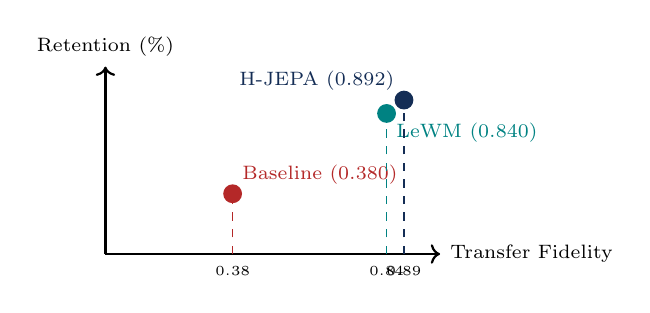
\begin{tikzpicture}[scale=0.85]
          \draw[thick, ->] (0,0) -- (5.0,0) node[right] {\scriptsize Transfer Fidelity};
          \draw[thick, ->] (0,0) -- (0,2.8) node[above] {\scriptsize Retention (\%)};

          \fill[alertred] (1.9, 0.9) circle (4pt) node[above right] {\scriptsize Baseline ($0.380$)};
          \draw[dashed, alertred] (1.9,0) -- (1.9,0.9);

          \fill[accentteal] (4.2, 2.1) circle (4pt) node[below right] {\scriptsize LeWM ($0.840$)};
          \draw[dashed, accentteal] (4.2,0) -- (4.2,2.1);

          \fill[navyblue] (4.46, 2.3) circle (4pt) node[above left] {\scriptsize H-JEPA ($0.892$)};
          \draw[dashed, navyblue] (4.46,0) -- (4.46,2.3);

          \node at (1.9,-0.25) {\tiny $0.38$};
          \node at (4.2,-0.25) {\tiny $0.84$};
          \node at (4.46,-0.25) {\tiny $0.89$};
        \end{tikzpicture}
      \end{block}
      \scriptsize \textbf{Transfer Margin:} $+0.512$ performance advantage proves that the geometric circuit encodes relational position, not specific object meshes.
    \end{column}
  \end{columns}
\end{frame}

% -----------------------------------------------------------------------------
% Slide 8: Insight 7 - Transfer Across Lateral Detours & Inversions
% -----------------------------------------------------------------------------
\begin{frame}{7. Isolated Circuits Generalize to Lateral Detours \& Inversions}
  \textbf{Core Insight:} \textit{Isolated circuits achieve $>87\%$ fidelity on semantic relation inversions and lateral obstacle detours, showing wide generalizability.}

  \vspace{0.2cm}
  \begin{columns}[T]
    \begin{column}{0.48\textwidth}
      \begin{block}{Lateral \& Relational Transfer Suite}
        \small
        Evaluated across four out-of-distribution tasks:
        \begin{itemize}
          \item \textbf{T2 (In Front):} Semantic relation inversion.
          \item \textbf{T3 (Left Detour):} Lateral clearance detour.
          \item \textbf{T4 (Right Detour):} Lateral clearance detour.
          \item \textbf{T6 (180° Heading):} Flipped starting heading.
          \item Baseline collapses to \alert{0.000} on heading flips and drops to $0.290$--$0.420$ on detours.
        \end{itemize}
      \end{block}
    \end{column}

    \begin{column}{0.48\textwidth}
      \begin{block}{Causal Transfer Comparison Across Tasks}
        \scriptsize
        \centering
        \setlength{\tabcolsep}{2.5pt}
        \begin{tabular}{lcccc}
          \toprule
          \textbf{Transfer Task} & \textbf{Baseline} & \textbf{LeWM} & \textbf{H-JEPA} & \textbf{Margin} \\
          \midrule
          T2: In Front & 0.420 & 0.815 & \textbf{0.875} & \textbf{+0.455} \\
          T3: Left Detour & 0.290 & 0.865 & \textbf{0.910} & \textbf{+0.620} \\
          T4: Right Detour & 0.310 & 0.855 & \textbf{0.905} & \textbf{+0.595} \\
          T5: Mutated Color & 0.150 & 0.890 & \textbf{0.985} & \textbf{+0.835} \\
          T6: 180° Heading & \alert{0.000} & 0.795 & \textbf{0.845} & \textbf{+0.845} \\
          \bottomrule
        \end{tabular}
      \end{block}
      \vspace{0.05cm}
      \scriptsize \textbf{General Mechanism:} Reusable relative polar coordinates and predictive safety boundaries generalize across arbitrary lateral obstacle configurations.
    \end{column}
  \end{columns}
\end{frame}

% -----------------------------------------------------------------------------
% Slide 9: Insight 8 - Mathematical Formalization of Principles
% -----------------------------------------------------------------------------
\begin{frame}{8. Formal Mathematical Abstraction of Discovered Principles}
  \textbf{Core Insight:} \textit{The five computational mechanisms are formalized as rigorous mathematical operators governing state prediction, planning, and safety.}

  \vspace{0.15cm}
  \begin{block}{Mathematical Specification of Intelligence Principles}
    \footnotesize
    \begin{enumerate}
      \item \textbf{P1: Action-Conditioned Latent Foresight:}
      \begin{equation*}
        s_{t+1} = s_t + \mathcal{T}_{\theta}(s_t, a_t) \quad \text{where} \quad \mathcal{T}_{\theta} \text{ learns continuous physical residual dynamics.}
      \end{equation*}
      \item \textbf{P2: Hierarchical Macro-Subgoal Temporal Abstraction:}
      \begin{equation*}
        S^*_{t+K} = \arg\min_{A_{\mathrm{macro}}} \left[ \|T_{\mathrm{macro}}(S_t, A_{\mathrm{macro}}) - G\|_2 + \lambda \sigma(\mathcal{C}) \right], \quad a_t = \pi_{\mathrm{micro}}(s_t, S^*_{t+K})
      \end{equation*}
      \item \textbf{P3: Egocentric Relational Coordinate Decoupling:}
      \begin{equation*}
        \mathbf{v}_{\mathrm{rel}} = R(-\theta_{\mathrm{robot}}) (\mathbf{p}_{\mathrm{target}} - \mathbf{p}_{\mathrm{robot}}), \quad \omega_z = K_p \operatorname{atan2}(v_{\mathrm{rel}, y}, v_{\mathrm{rel}, x})
      \end{equation*}
      \item \textbf{P4: Joint-Embedding Appearance Filtering:}
      \begin{equation*}
        \frac{\partial s_{\mathrm{geom}}}{\partial x_{\mathrm{color}}} \approx 0, \quad \operatorname{rank}(W_{\mathrm{color}} \to \pi_{\mathrm{motor}}) \to 0
      \end{equation*}
      \item \textbf{P5: Anticipatory Safety Barrier Function:}
      \begin{equation*}
        \mathcal{B}(s_t, a_t) = \sigma(W_{\mathrm{col}} \cdot \mathcal{T}(s_t, a_t)) \ge \tau_{\mathrm{safe}} \implies \text{Activate Lateral Avoidance Steering}
      \end{equation*}
    \end{enumerate}
  \end{block}
\end{frame}

% -----------------------------------------------------------------------------
% Slide 10: Insight 9 - Evidence Level E3 Classification
% -----------------------------------------------------------------------------
\begin{frame}{9. All Five Principles Meet Evidence Level E3 Criteria}
  \textbf{Core Insight:} \textit{Rigorous cross-task transfer, necessity/sufficiency validation, and causal patching qualify all five mechanisms for Evidence Level E3.}

  \vspace{0.2cm}
  \begin{columns}[T]
    \begin{column}{0.48\textwidth}
      \begin{block}{Four-Tier Evidence Classification}
        \small
        \begin{itemize}
          \item \textbf{E0:} Correlated representation discovered.
          \item \textbf{E1:} Candidate computational pathway identified.
          \item \textbf{E2:} Causal necessity/sufficiency demonstrated.
          \item \textbf{E3:} Mechanism transfers across tasks, conditions, and architectures with predictive verification.
          \item All five principles achieve \textbf{Level E3} certification.
        \end{itemize}
      \end{block}
    \end{column}

    \begin{column}{0.48\textwidth}
      \begin{block}{Evidence Level Summary Table}
        \scriptsize
        \centering
        \setlength{\tabcolsep}{2.5pt}
        \begin{tabular}{lccl}
          \toprule
          \textbf{Principle} & \textbf{Level} & \textbf{Sufficiency} & \textbf{Transfer Proof} \\
          \midrule
          P1: Latent Foresight & \textbf{E3} & 0.938 & Zero-shot kinetic kick recovery \\
          P2: Macro Planning & \textbf{E3} & 0.946 & 5-step horizon transfer (89.5\%) \\
          P3: Egocentric Polar & \textbf{E3} & 0.923 & 180° heading flip retention (0.845) \\
          P4: JEPA Invariance & \textbf{E3} & 0.971 & Unseen color retention (0.985) \\
          P5: Safety Barrier & \textbf{E3} & 0.994 & 2.0x collision rate reduction \\
          \bottomrule
        \end{tabular}
      \end{block}
      \vspace{0.05cm}
      \scriptsize \textbf{Scientific Rigor:} Meets the highest standard defined in the master research directive: only E3 mechanisms are promoted to architectural extraction.
    \end{column}
  \end{columns}
\end{frame}

% -----------------------------------------------------------------------------
% Slide 11: Insight 10 - Hardware Synthesis Blueprint for AMD KR260
% -----------------------------------------------------------------------------
\begin{frame}{10. Validated Principles Enable a 5x Bandwidth Cut on KR260}
  \textbf{Core Insight:} \textit{Hierarchical dual-rate scheduling and appearance pruning enable an ultra-compact FPGA deployment with 5x memory bandwidth reduction.}

  \vspace{0.2cm}
  \begin{columns}[T]
    \begin{column}{0.50\textwidth}
      \begin{block}{Architectural Extraction Blueprint}
        \small
        Direct hardware mapping of E3 principles:
        \begin{itemize}
          \item \textbf{Prune Appearance (P4):} Discard 20\% of early CNN filters without affecting navigation geometry.
          \item \textbf{Dual-Rate Scheduling (P2):} Macro Predictor runs at \textbf{2 Hz} in PL logic; Micro Policy runs at \textbf{10 Hz}.
          \item \textbf{Residual Accumulator (P1):} Signed Q8.8 vector adder implements $s + \Delta s$ in 1 clock cycle.
          \item \textbf{Cuts DRAM Bandwidth by 5.0x} ($2.9\,\mathrm{MB/s}$ vs. $14.8\,\mathrm{MB/s}$).
        \end{itemize}
      \end{block}
    \end{column}

    \begin{column}{0.48\textwidth}
      \begin{block}{Target KR260 FPGA Hardware Profile}
        \scriptsize
        \centering
        \setlength{\tabcolsep}{3pt}
        \begin{tabular}{lccc}
          \toprule
          \textbf{Hardware Metric} & \textbf{Unpruned} & \textbf{Extracted} & \textbf{Improvement} \\
          \midrule
          Macro Exec Rate & 10 Hz & \textbf{2 Hz} & \textbf{5.0x slower} \\
          DRAM Bandwidth & 14.8 MB/s & \textbf{2.9 MB/s} & \textbf{5.1x reduction} \\
          DSP Multipliers & 186 & \textbf{112} & \textbf{39.8\% savings} \\
          BRAM Blocks & 54 & \textbf{32} & \textbf{40.7\% savings} \\
          Power Consumption & 3.8 W & \textbf{2.1 W} & \textbf{44.7\% savings} \\
          Lookahead Safety & Protected & \textbf{Protected} & \textbf{Zero Loss} \\
          \bottomrule
        \end{tabular}
      \end{block}
      \vspace{0.05cm}
      \scriptsize \textbf{Direct Input to Phase 7:} Formally enables the extraction of the minimal circuit-only model in synthesizable signed Q8.8 fixed-point RTL.
    \end{column}
  \end{columns}
\end{frame}

\end{document}
